\chapter{System Identification in the frequency domain}
This section describes various system identification procedures in the frequency domain. We'll start with the openloop identification of the bicycle only. This can be of use when validating the bicycle equations. This is done for both the SISO and more general MIMO case. Later on similar techniques will be applied for identifying the human controller. Here we assume the bicycle dynamics to be  a known system and solve for the 'unknown' human controller.
\section{General strategy}
The system identification procudures will be tested using simulink models. This offers a both controllable and flexible enviroment where measurement uncertainties are simply modelled using white noise. The systems subject to identification $H$ are actually known at forehand and are used to verify the estimated system $\hat{H}$. The goal of these simulations is to find a usefull identification procudure for the real experiments. 
\section{Input signal design}
In this section, some commonly used perturbation signals will be discussed. An overview is given at the end of this section.
\subsection{White noise}
A continues white noise input ${u(t)}$ is characterized by the following properties;
	\begin{align}
			\mu_u &= E\{{u}(t)\} = 0  \\
			R_{uu} &= E\{{u}(t_1){u}(t_2)\} = \tfrac{1}{2}N\delta(t_1-t_2)
	\end{align}
Which basically means that the input $\mathbf{u}$ has zero mean ($\mu_u$) and each of the input indices are uncorrelated ($R_{uu}$) with each other. $N$ represents the number of samples and is infinite in a continues signal. Notice that the fourier transformation of a delta dirac function $\delta(t_1-t_2)$ gives simply one, the expected autospectral density of the white noise signal thus simply becomes;
	\begin{align}
			E\{S_{uu}\} = \tfrac{1}{2}N
	\end{align}
This is a very nice but strange property. It is nice because the average spectral density stays constant for all frequencies, allowing for infinite bandwidth identification. It also is a strange property, because this signal appears to have infinite power. However in practice we use discrete signals, which results in a finite bandwidth and thus finite power. In addition, we also may choose to apply a low pass filter to limit the frequency content to a certain range of interest.
		White noise is a random process, which makes it is impossible to predict future values. This is a nice property when identifying the human controller, since humans are capable of adapting their control strategy. Using random variables thus eliminates the possibility of using feedforward control. This assumption can be checked afterwards by analyzing the input ($y$) and output ($y$) covariance $C_{yu}$ as a function of the time difference $\tau$ between the two signals. 
	\begin{align}
			C_{yu} (\tau) = 0 \ \ , \ \tau < 0  
	\end{align}
This means that the output only depends on previous inputs, i.e. there exists a causal relationship between input (cause) and output (causality).
\subsection{Sine sweep}
The sine sweep is often used for structual vibration analsyis. Here the model subject to identification, is excited using a sine sweep, which most of the time starts at at low frequency and gradually builds up to higher frequencies. A typical definition of the swept sine is given by;
	\begin{align}
			u(t) = 2A\sin\left(\left[\pi(f_\textrm{max}-f_\textrm{min})\frac{t}{T} + 2\pi f_\textrm{min}\right] t\right)
	\end{align}
The autospectral density of this signal is constant between $f_\textrm{min}$ and $f_\textrm{max}$ and gradually decreases at $f>f_\textrm{max}$.
		Unfortuneatly the swept sine is a highly predictive signal, allowing a human controller to make use of feed forward control.
\subsection{Random phase multisine}
Finally we introduce the random phase multisine. Here we start by constructing the signal in the frequency domain and then convert the signal back to the time domain using a inverse Fourier transformation. The random multisine can be defined as follows:
	\begin{align}
			|U(\omega)| &= \begin{cases} 1 & \mathrm{for}  \ \omega_\textrm{min} \le \omega \le \omega_\textrm{max}, \\ 0 & \mathrm{for}\ \omega > \omega_\textrm{max} \end{cases}  \\
			\angle U(\omega) &= \begin{cases} \theta & \mathrm{for}  \ \omega_\textrm{min} \le \omega \le \omega_\textrm{max}, \\ 0 & \mathrm{for}\ \omega > \omega_\textrm{max} \end{cases}  
	\end{align}
Where $\theta$ is randomly distributed for each frequency $\omega$ according to an uniform probability density function.
Setting up signals in the frequency domain allows for easy autospectral density shaping. This is a nice feature, because we are generally interested in the frequency content of the input signal. Using this method allows the user to select one or multiple desired frequency bands. Unfortuneatly this kind of signal modelling in the frequency domain may result in unwanted peaks in the time domain.
\subsection{Crested multisine}
To reduce peak amplitudes while mainting the desired average power density, the phase can be optimized to fullfill these properties. The crest factor forms a usefull definition when optimizing the signal;
\begin{align}
    C = \frac{u_\textrm{max}}{u_\textrm{rms}} = \frac{\max(\mathbf{u})}{\sqrt{N^{-1}\mathbf{u}^T\mathbf{u}}}
\end{align}
The objective function will be to reduce the crest factor, the parameters subject to optimization will be the phase indices. It is beyond the scope of this report to explain the optimization algorithm in detail. What is important is that the resulting signal indeed has a significant lower crest factor. 
\subsection{Comparison}
A short overview of the various input signals is given in table.
		\begin{figure}
			\centering
				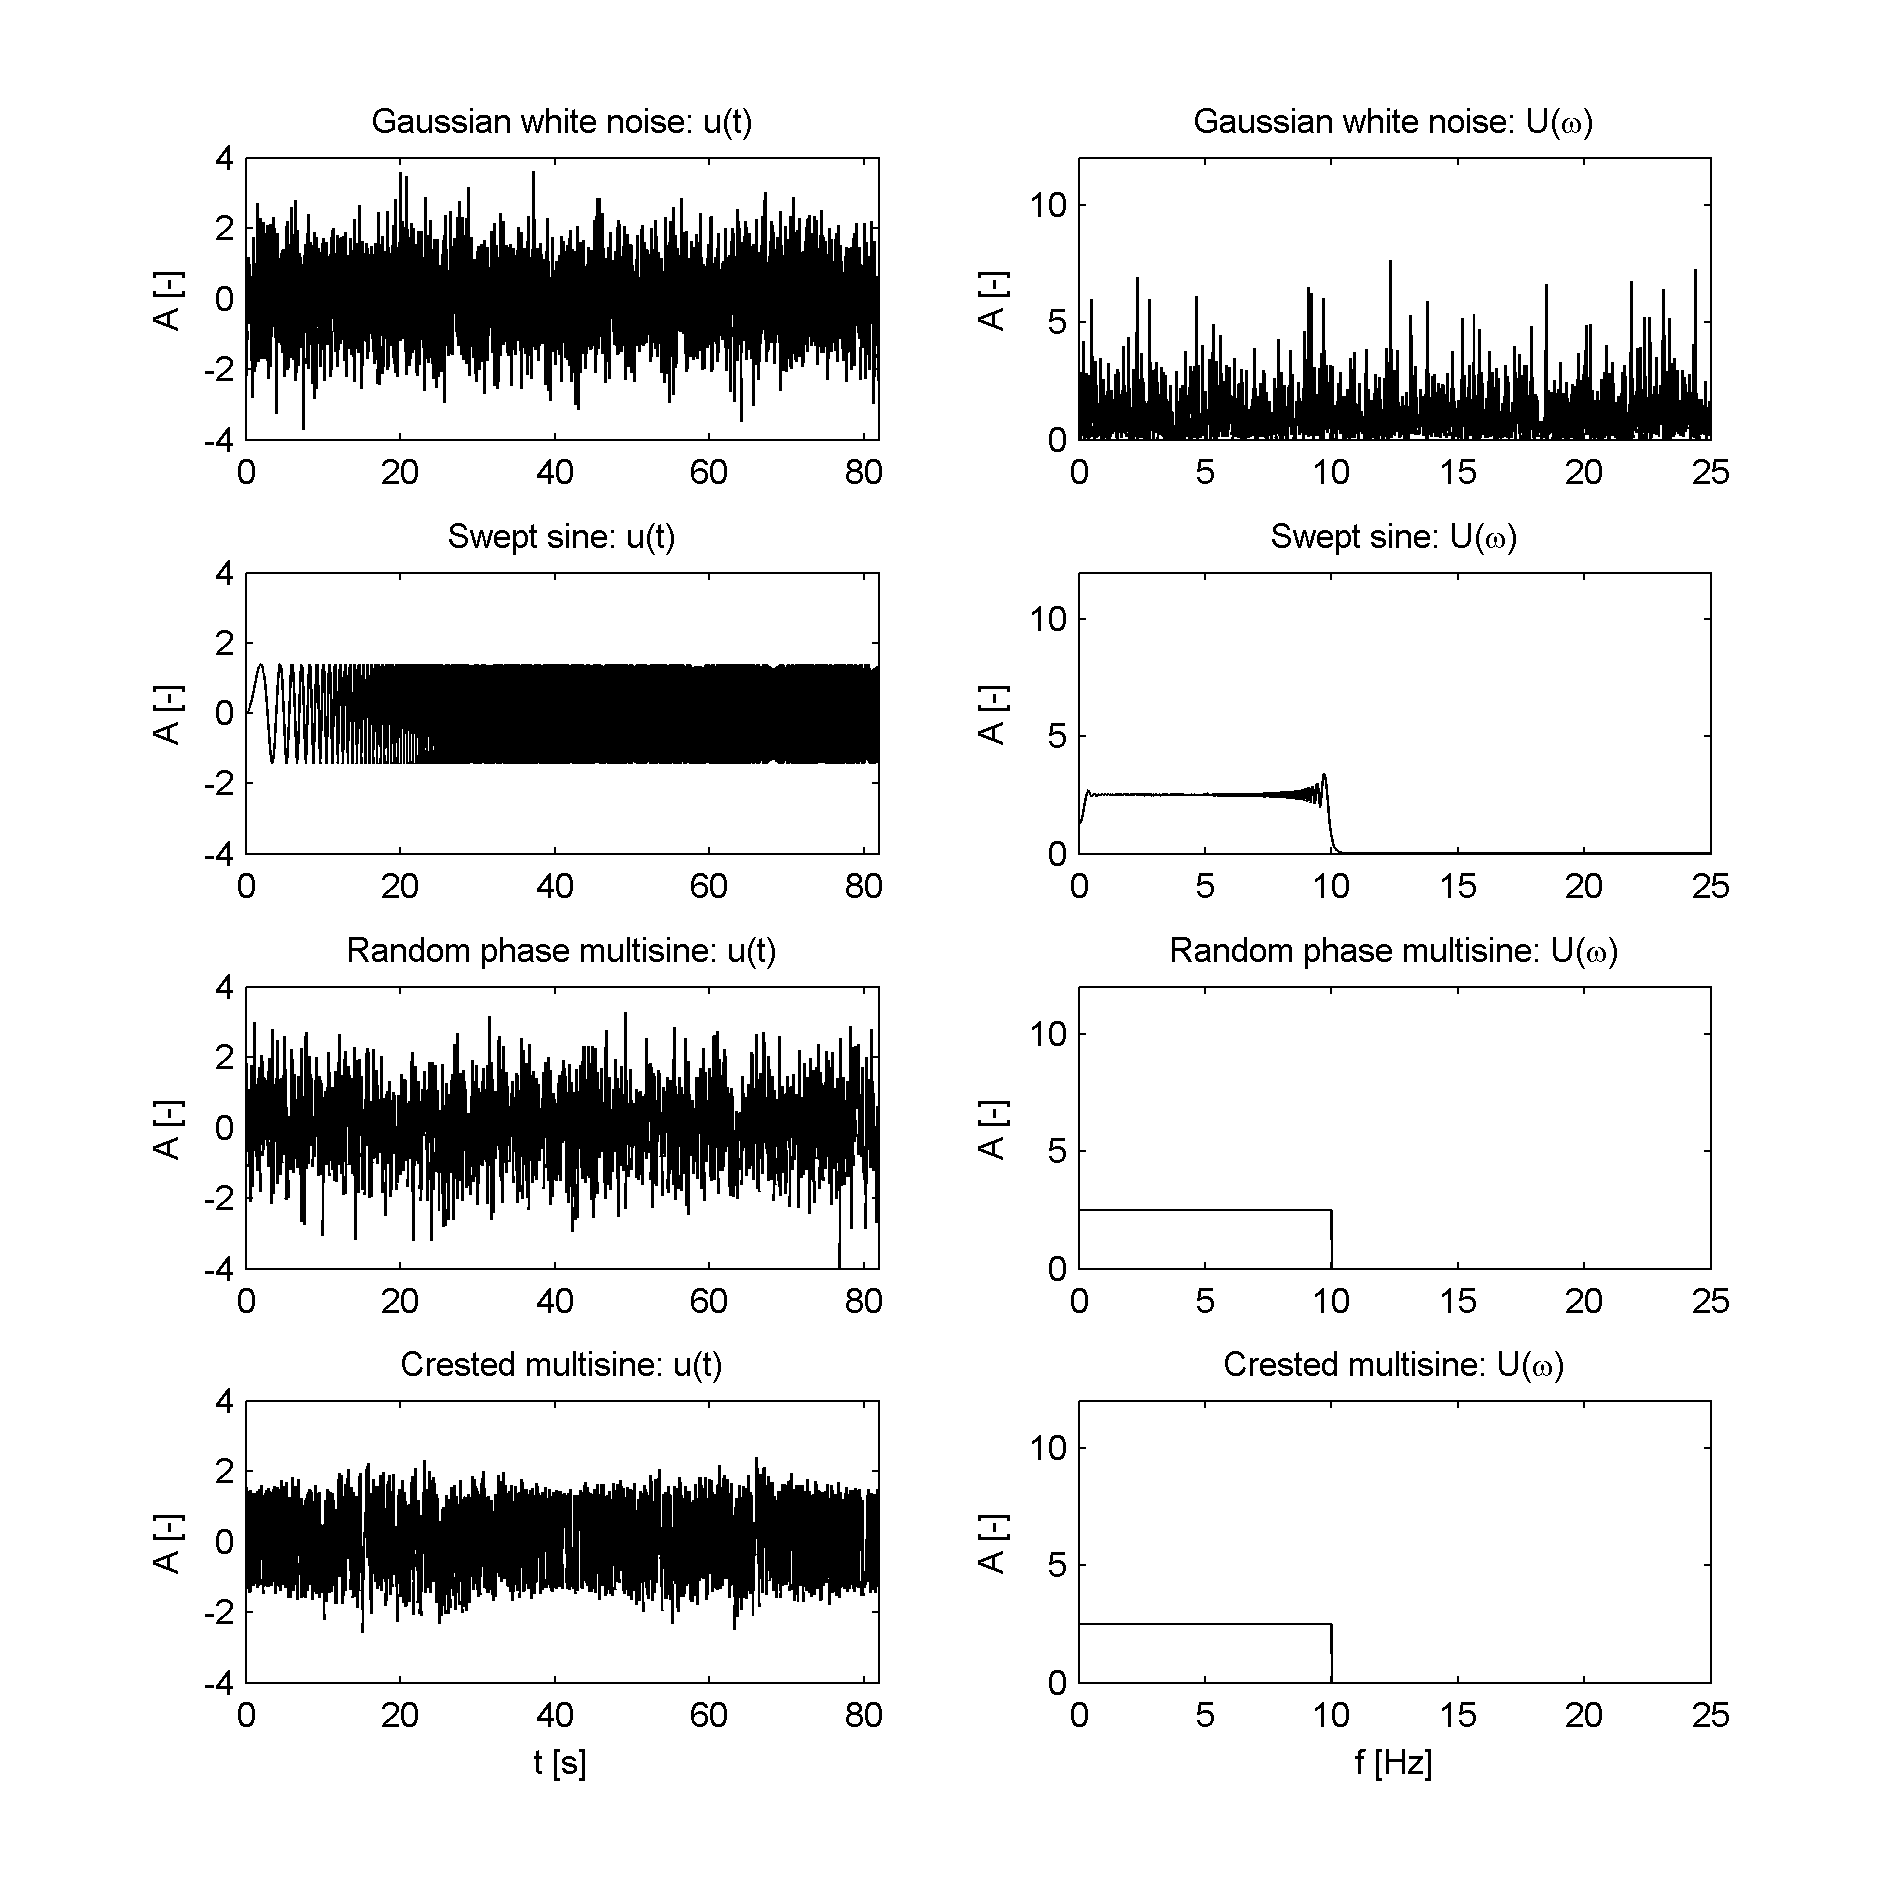
\includegraphics{images/u}
			\label{fig:u}
			\caption{4 different input signals: Gaussian white noise, swept sine, random phase multisine, crested random phase multisine}
		\end{figure}
\begin{table}
		\centering
		\begin{tabular}{lrrrr}
		\toprule
																			& White noise & Swept sine & Multisine & Crested  \\
		\midrule
		Mean ($\mu_u$):					& 0 & 0 & 0 & 0 \\
		Correlation ($R_{uu}$):	& 1 & 1 & 1 & 1 \\
		Spectral density ($S_{uu}):$ 										& 1.0145 &   2.4912  &  2.5000  &  2.5000 \\
		Crest factor ($C$): 						& 3.6129   & 1.4026  &  3.2857   & 2.3943 \\
		Predictable: 								& no & yes & no & no \\
		\bottomrule
		\end{tabular}
		\label{table:u}
		\caption{Comparison of various input signals. Notice that the spectral density is defined as the average spectral density over the desired frequency band.}
\end{table}
\subsection{Results}
The multisine offers the best results, but is predicatable, therefore the crested multisine is advised when identifying  the human controller.
\section{Frequency averaging}
Frequency averaging is used to reduce the influence of noise in the frequency domain at the cost of a decreased frequency resolution. There are 2 commonly used methods for frequency averaging; frequency block averaging and averaging over neighbouring frequencies. Yet to be described in more detail. 
\section{SISO identification}
Suppose we measure both the steering torque $T_\delta$ and roll angle $\phi$. This can be modelled as a simple open loop, single input, single output system. This corresponding block diagram is shown below:
%\begin{figure}{h!}
	\begin{center}
		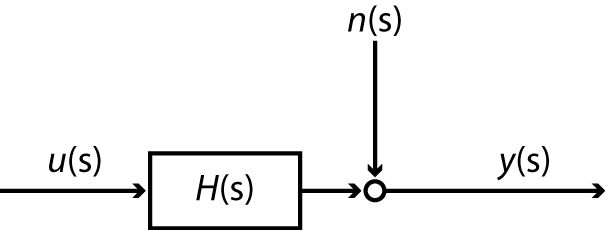
\includegraphics{images/SISOblock}
		%		\caption{Blockdiagram of the SISO model}
		\label{fig:SISOblock}
	\end{center}
	Where $u = u(s)$ represents the steering torque $T_\delta$ input, $\hat{y}= y(s)$ represents the measured output and $n= n(s)$ represents the measurement noise. 
\subsection{Simulation}
The linearized benchmark equations are used for the simulation. A forward velocity of 5 m/s is chosen, which results in stable dynamic behavior of the bicycle. The transferfunction from steering torque $T_\delta$ to roll angle $\phi$ is derived and yields (in zero-pole-gain form):
\begin{align}
H =   \frac{  -0.12262 (s+58.91) (s+13.77)  }{ (s+0.35) (s+14.27) (s^2 + 1.594s + 19.53) } 
\end{align}
This model will be used to simulate the bicycle response. Later on we will assume the system to be unknown and use system identification and parameter estimation techniques to estimate the  transfer function. Naturally the following question arises; ''why bother estimating a system that is already known?'. De answer to this this question is that we are actually interested in the quality of the identification procedures. The quality of the estimated fit can easily be checked by comparing it with the true system.

A simulation is set up, using the following measurement parameters:
			\begin{center}
				\begin{tabular}{lccc}
				\toprule
				description & symbol & value & units  \\
				\midrule
					Measurement time	 &	T    					& $100	$							& [s] 		\\
					Sample frequency	 &		$f_s$   			& $50		$							& [Hz] 	\\
					Sample period				 &	$\Delta T$ & $1/f_s$ 							& [s] 		\\
					Number of samples &		$N$    			& $T/\Delta T	$			& [-]			\\
					Input bandwidth & $f_{bw}$ & $2$                   & [Hz] \\
					\bottomrule
				\end{tabular}
			\end{center}
The input signal $u$ is designed as an crested multisine, which is described in the previous chapter. The maximum torque is set to 0.6 Nm. The standard deviation of the noise is set to 0.01 rad.
Next the simulation is started resulting in the measured output $y(t)$. The input and output are then converted to the frequency domain, spectral densities are calculated and finally some frequency averaging (not discussed) is applied in order to reduce the noise.
\subsection{System identification}
Next we will use the simulated dataset to derive the transfer function of the system. Starting from the block diagram shown in figure \ref{fig:SISOblock} we can derive the following equation:
\begin{align}
		Hu & = y-n 
\end{align}
Unfortuneatly we don't know the the noise $n$, which makes solving for $H$ impossible. However we can find a linear estimation of the system by seeking a solution under the image of $u$. This is achieved by projecting $u$ onto the left side of the equations. Assuming the noise is uncorrelated with the input (they are 2  independent signals), the linear estimated transferfunction $\hat{H}$ can be derived:
\begin{align}
		u^\ast Hu & = u^\ast (y-n) \nonumber \\
		H 					& = \frac{u^\ast (y-n)}{u^\ast u}  \nonumber \\
		\hat{H}	& = \frac{u^\ast y}{u^\ast u} \nonumber \\
		\hat{H} 	& = \frac{S_{uy}}{S_{uu}}
		\label{eq:SISOH}
\end{align}
Here $S_{uy}$ represent the cross spectral density of the input/output and $S_{uu}$ represents the auto spectral density of the input. The resulting tranferfunction is shown as a bode function in figure \ref{fig:SISObode}. The gain of the transfer function decreases as the frequency increases, resulting in a poorer signal to noise ratio at higher frequencies. Also notice that the input signal contains frequency content ranging from 0 to 2 Hz. Above 2 Hz the response is dominated completly by the noise. The coherence represents the linear estimation quality of the transfer function. As expected, the coherence drops dramatically above 2 Hz.
	\begin{figure}
		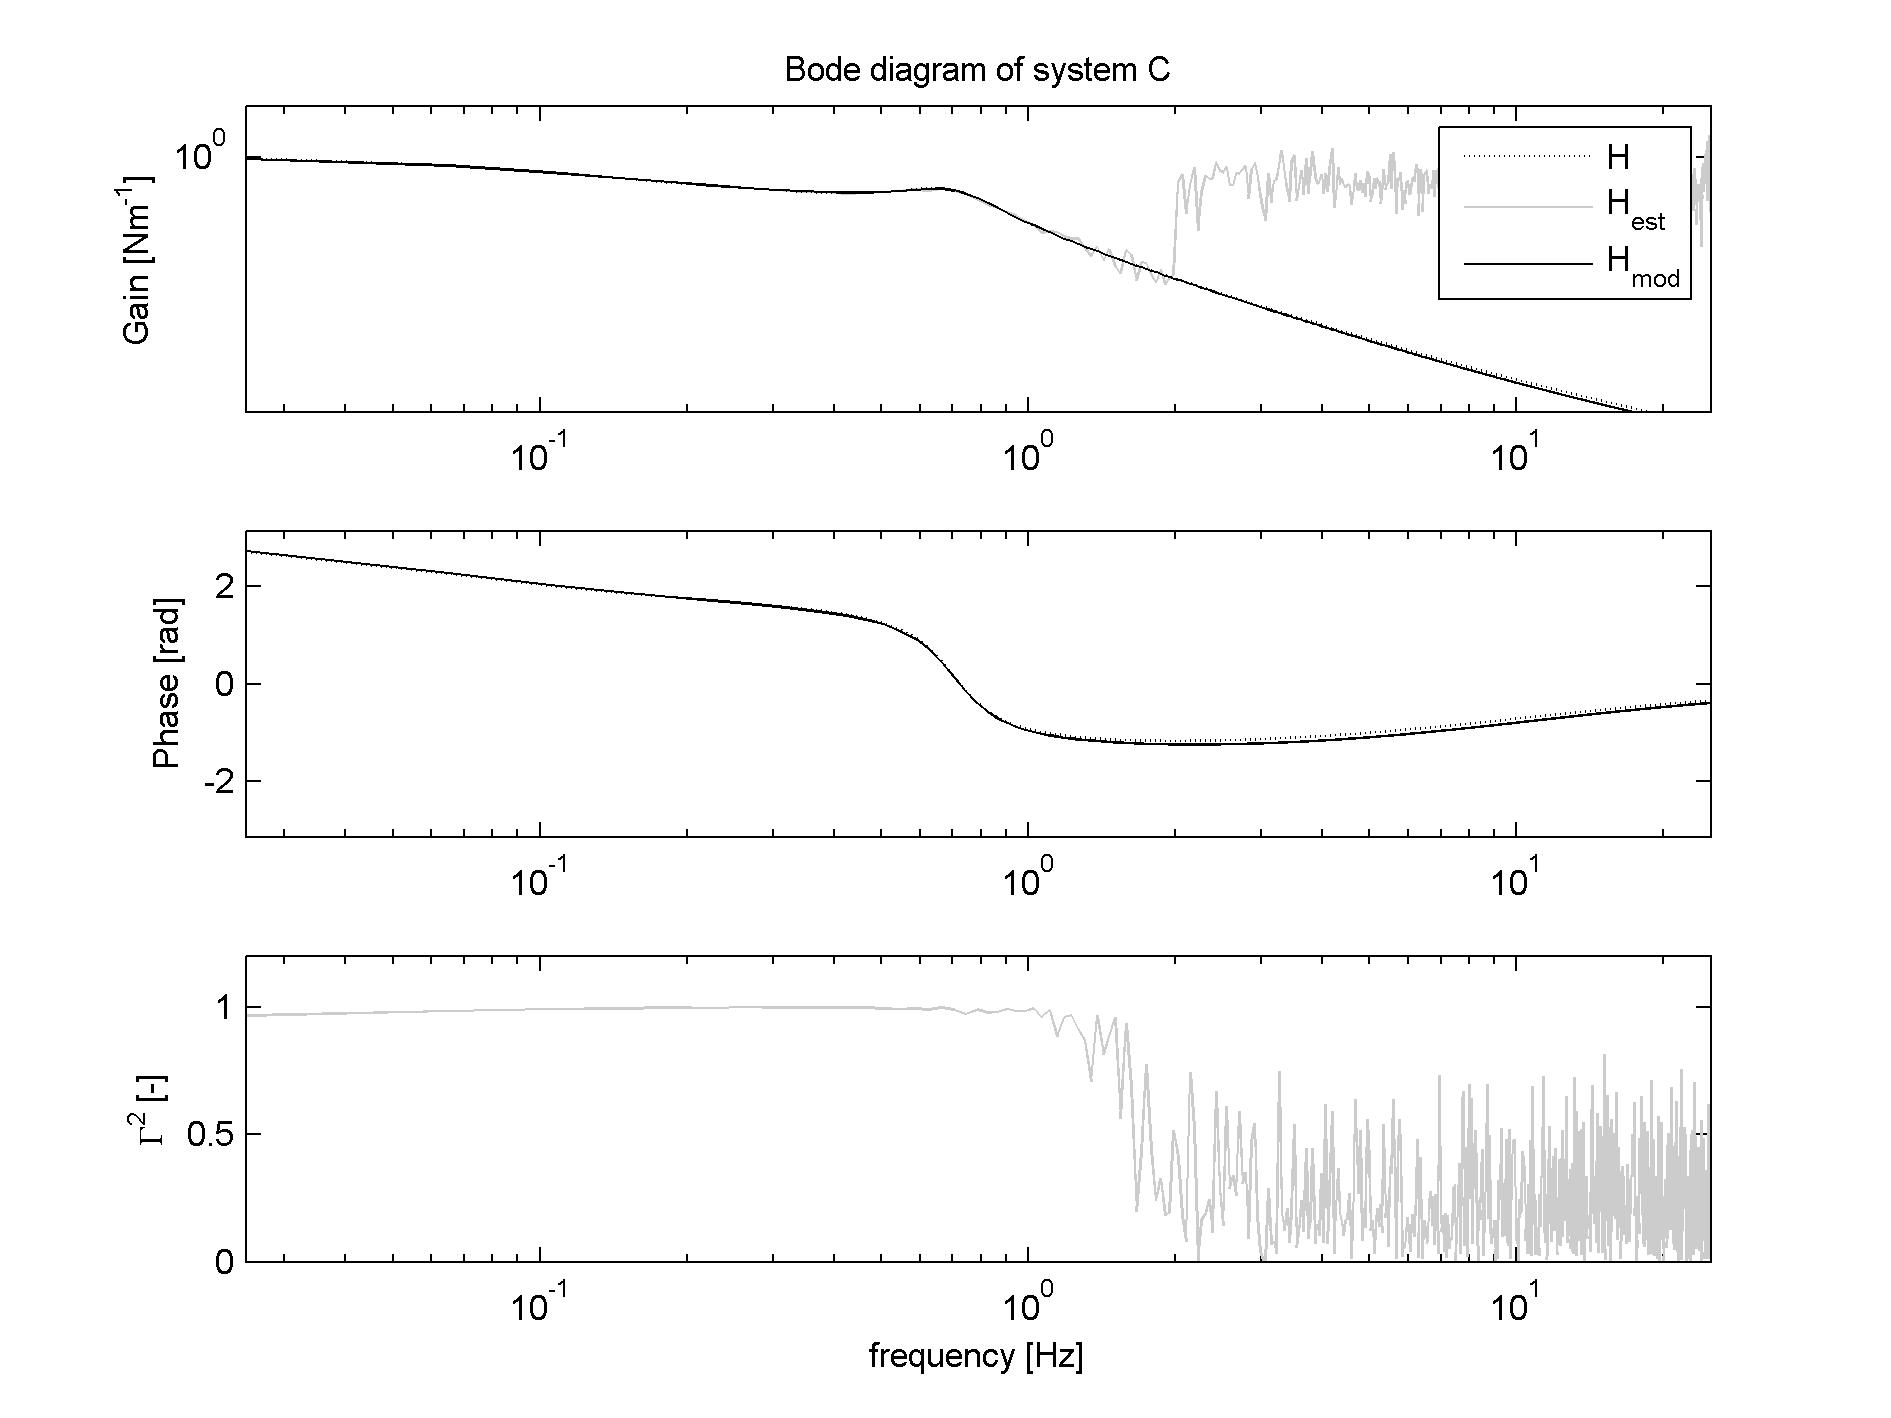
\includegraphics{images/SISObode}
		\caption{Bode diagram of the true ($H$), estimated ($H_{est}$) and parametric ($H_{mod}$) transfer function.}
				\label{fig:SISObode}
	\end{figure}
\subsection{Parameter estimation}
The estimated tranferfunction can then be used to determining the actual parameters of the transferfunction. We assume a solution of the following form:
	\begin{align}
		H_{\textrm{mod}}(s,x_i) = \frac{ x_1 (s+x_2) (s+x_3)  }{ (s+x_4) (s+x_5) (s^2 + x_6s + x_7) } 
	\end{align}
The error function is chosen to be:
		\begin{equation}
		e_s = \sqrt{\frac{1}{2\pi\omega_s}}\gamma(\omega_s)\left|\ln \hat{H}(\omega_s)-\ln H_{mod}(\omega_s,x_i)\right|
		\end{equation}
Here the $1\omega$ term acts as a weightening function, which puts more weight on lower frequencies. The $\ln$ function puts more weight on errors at lower magnitudes. This error definition is commonly used when fitting in the frequency domain. The reason to use these special weightnings is to counteract the logarithmic scale of a bode magnitude plot.
The criterium thus becomes:
		\begin{equation}
		J = \frac{1}{2}\sum_{s} e_s^2
		\end{equation}	
The Matlab \mcode{lsqnonlin} algorithm is used for the optimization. The resulting parameters together with the true parameters are shown in table \ref{table:SISOparms}.
\begin{table}
\centering
		\begin{tabular}{cccc}
		\toprule
		$x_i$ & True & Estimated & $\sigma_{\mu_{x_i}}$ \\
		\midrule
		$x_1$&   -0.1112  	& -0.1226  	&  0.1241\\
		$x_2$&	58.0972   	&58.9100  	& 89.8280\\
    $x_3$&	7.3382   		&13.7700  	& 35.0404\\
    $x_4$&	0.3715   		& 0.3500  		&  0.0295\\
    $x_5$&	6.6603   		&14.2700  	& 29.0601\\
    $x_6$&	1.5845    	&1.5940  		&  0.1576\\
		$x_7$&	19.7927  	&19.5300 		&   0.6974\\
		\bottomrule
 		\end{tabular}
		\caption{Comparison of the estimated parameters with the true parameters. $\sigma_{\mu_{x_i}}$ represents the standard deviation of the mean.}
		\label{table:SISOparms}
\end{table}
The quality of the resulting parameters is varying. Some parameters ar more difficult to fit than others. When we look at the true system (equation \ref{eq:SISOH}), we observe a near zero/pole cancelation of the 3th and 5th parameter, which renders them practically unobservable. This makes these parameters very hard to  fit, which results in a huge uncertainty in the estimation these 2 corresponding parameters. The low quality fit of parameter 2 is unknown at this point. Possibly the optimization algorithm got stuck on a global minimum. The resulting fit (shown in figure \ref{fig:SISObode} seems pretty good however.
\section{MIMO identification}
Next we are interested in estimating the complete bicycle equations. The system has two inputs; rolling torque $T_\phi$ and steering torque $T_\delta$. The following outputs are measured; roll angle $\phi$ and steerangle $\delta$. Since the system has multiple inputs and multiple outputs we have to apply MIMO system identification techniques. The corresponding block diagram is shown below:
	\begin{center}
		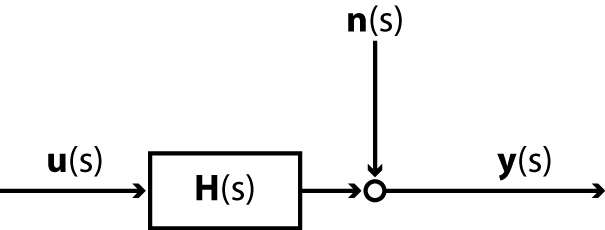
\includegraphics{images/MIMOblock}
		%		\caption{Blockdiagram of the SISO model}
		\label{fig:MIMOblock}
	\end{center}
Where $\mathbf{u} = \mathbf{u}(s)$ represents the input vector, $\mathbf{y}= \mathbf{y}(s)$ represents the measured output vector and $\mathbf{n} = \mathbf{n}(s)$ represents the measurement noise vector. The block diagram looks pretty similar to the SISO case, except here the scalar function are replaced by vectors and matrices.
\subsection{Simulation}
Again the linearized benchmark equations are used for the simulation. A forward velocity of 5 m/s is chosen, which results in stable dynamic behavior of the bicycle. The governing input/output relationship is shown below in state space form:
	\begin{align}
		\mathbf{\dot{x}} & = \mathbf{A}\mathbf{x} + \mathbf{B}\mathbf{u} \nonumber \\
		\mathbf{y} & = \mathbf{C}\mathbf{x} 
	\end{align}
Where;
	\begin{align}
	{\scriptstyle
			\mathbf{A} =   \left[\begin{array}{cccc} 
									$0$ & $0$ & $1$ & $0$ \\
									$0$ & $0$ & $0$ & $1$ \\
									$9.470$ & $-22.758$ & $-0.520$ & $-1.638$ \\
									$12.400$ & $-19.499$ & $18.089$ & $-15.694$   
			\end{array}\right]   \nonumber \ \ , \
			\mathbf{B} = \left[\begin{array}{cc}
									 $0$ & $0$ \\
									$0$ & $0$ \\
									$0.016$ & $-0.123$ \\
									$-0.123$ & $4.265$ 
			\end{array}\right] \nonumber \ \ , \ 
			\mathbf{C} = \left[\begin{array}{cccc}
									$1$ & $0$ & $0$ & $0$ \\
									$0$ & $1$ & $0$ & $0$
			\end{array}\right]  \nonumber
	}
	\end{align}
A simulation is set up, using the same measurement parameters as for the SISO case (see table: \ref{table:SISOparms}. The input signal $\mathbf{u}$ is designed as an crested multisine which will be explained later on in more detail. The maximum steering torque is set to 0.6 Nm and the maximum roll torque is set to 10 Nm. The standard deviation of the noise for all measured outputs is set to 0.01 rad. The simulation is run twice, with different input vectors. 
\subsection{MIMO system identification}
Next we will use the simulated dataset to derive the transfer function of the system. Starting from the block diagram shown in figure \ref{fig:MIMOblock} we can derive the following equation:
\begin{align}
		\mathbf{H}\mathbf{u} & = \mathbf{y}-\mathbf{n} 
\end{align}
Unfortuneatly this system is not solvable, since we can't invert the inputvector $\mathbf{u}$. Therefore we need additional measurements. A nice choice of input would be the following:
\begin{align}
		\mathbf{U}(s) = \left[\begin{array}{cc}
									A_\phi &  A_\phi \\
									A_\delta & -A_\delta \\
			\end{array}\right] u(s)
\end{align}
Where $A_\phi=5$ and $A_\delta=0.6$ are amplification gains which are found by trial and error. Similar as in the SISO case we will seek a solution in the image of $\mathbf{U}$. Here only need to be a little bit more carefull, since the multiplication of vectors and matrices is generally non-communicative.
\begin{align}
		\mathbf{H}\mathbf{U} & = \mathbf{Y}-\mathbf{N}  \nonumber \\
		\mathbf{U}^\ast\mathbf{H}^\ast & = \mathbf{Y}^\ast-\mathbf{N} ^\ast \nonumber \\
			\mathbf{U}\mathbf{U}^\ast\mathbf{H}^\ast & = 	\mathbf{U}\left(\mathbf{Y}^*-\mathbf{N} ^\ast\right) \nonumber \\
			\mathbf{H}^\ast & = 	\left(\mathbf{U}\mathbf{U}^\ast\right)^{-1}\mathbf{U}\left(\mathbf{Y}^\ast-\mathbf{N} ^\ast\right) \nonumber \\
						\mathbf{H} & = 	\left(\mathbf{Y}-\mathbf{N}\right)\mathbf{U}^\ast\left(\mathbf{U}\mathbf{U}^\ast\right)^{-1} 
\end{align}
Next we define the estimated transferfunction $\hat{\mathbf{H}}$ to be the transferfunction that linearly correlates the input/output data, assuming that the input is independent of the noise ($\mathbf{N}\mathbf{U}^\ast \approx \mathbf{0}$). 
\begin{align}
						\hat{\mathbf{H}} 	= & \mathbf{Y}\mathbf{U}^\ast\left(\mathbf{U}\mathbf{U}^\ast\right)^{-1} \nonumber \\
																			= & \mathbf{S}_{yu}\mathbf{S}_{uu}^{-1}
		\label{eq:MIMOH}
\end{align}
Here $S_{uy}$ represent the cross spectral density of the input/output and $S_{uu}$ represents the auto spectral density of the input. The resulting tranferfunction is shown as a bode function in figure \ref{fig:SISObode}. The gain of the transfer function decreases as the frequency increases, resulting in a poorer signal to noise ratio at higher frequencies. Also notice that the input signal contains frequency content ranging from 0 to 2 Hz. Above 2 Hz the response is dominated completly by the noise. The coherence represents the linear estimation quality of the transfer function. As expected, the coherence drops dramatically above 2 Hz.
	\begin{figure}
		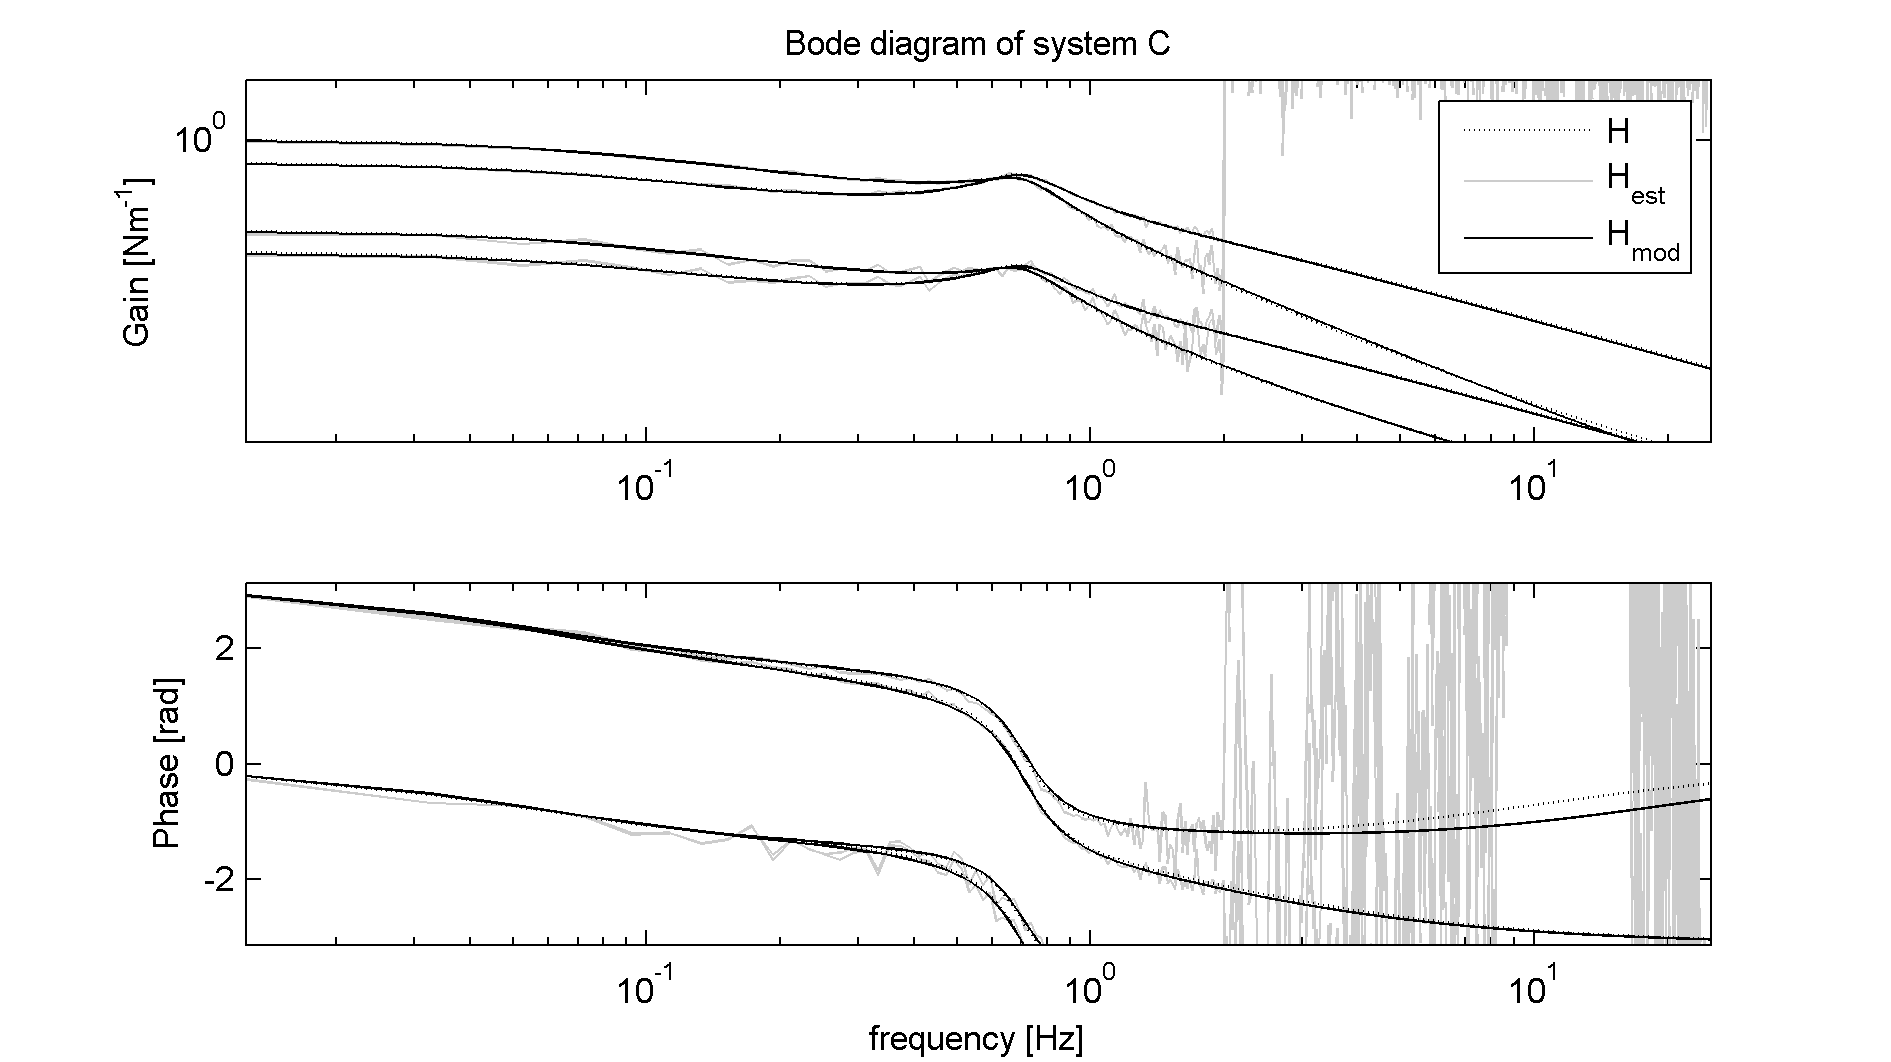
\includegraphics{images/MIMObode}
		\caption{Bode diagram of the true ($H$), estimated ($H_{est}$) and parametric ($H_{mod}$) transfer function.}
				\label{fig:MIMObode}
	\end{figure}
	\subsection{MIMO parameter estimation}
	Yet to be done.
